\section{Open-Source Numerical Shear Wave Solvers}\label{sect:open_source}

\subsection{FEBio (Dr. Jiang)}
FEBio~\cite{Mass2012} models orresponding to three Phase II CIRS phantom
materials (E2297-AX, E2297-BX and E2297-CX) have been generated. Quasi-linear
viscoelastic material properties and an acoustic pushing beam based on a
published paper from Dr.  Palmeri’s work~\cite{Palmeri2008} have been assigned
to each numerical model.  Those models were used to investigate estimation of
shear wave (SW) phase velocity and SW dispersion. Those FEBio models contain
1.0--1.5 million tetrahedral elements and take approximately 6 hours to solve
for a high-end, multi-core workstation (12 cores, 64 GB memory, Ubuntu 12.04).
Subsequently, simulated SW data were analyzed to obtain phase velocity values
and their frequency dependence.

There were three tasks in this effort:

\begin{description}
    \item[Task 1:] Simulate acoustic pushing pulse
        The following conditions were simulated, consistent to the early
        publication by Dr.  Palmeri~\cite{Palmeri2008}:
        \begin{itemize}
            \item Acoustic pressure pulses of a typical curvilinear transducer (Siemens 4C1)
            \item F/2 and center frequency of 2.3 MHz
            \item One focal depth at 30 mm
            \item Measured pressure pulses by hydrophones (by Duke) were applied
            \item One cycle of the sinusoidal pulse was applied
        \end{itemize}
    \item[Task 2:] Fit material properties using a Quasi-linear Viscoelastic
    (QLV) model available in FEBio~\cite{Weiss2012}
        
    Viscoelasticity of soft tissues was taken into consideration by a
    quasi-linear viscoelastic (QLV) material model~\cite{Fung1993a} implemented
    in FEBio.  In the quasi-linear viscoelastic model, a relaxation function
    G(t) was used~\cite{Gerig2003} to simulate time dependent behaviors as
    follows,

    \begin{equation}\label{eqn:qlv}
        G(t) = 1 + \sum\limits_{i=1}^N \gamma_i \exp\left(\frac{-t}{\tau_i}\right)
    \end{equation}

    where $\tau_i$ represents one of relaxation time values in the Prony
    series, and $\gamma_i$ is the viscoelastic coefficient in the Prony series.
    In this study, $N$ was set to be 1 and (\ref{eqn:qlv}) became a
    three-element Standard Linear Solid (SLS) model (Figure~\ref{fig:sls}).
    Parameters of three CIRS materials (E2297-AX, E2297-BX and E2297-CX) have
    been fitted into the above-mentioned relaxation function (\ref{eqn:qlv}).
    The elastic contributions to the quasi-linear viscoelastic material model
    are being simulated using the well-known Neo-Hookean model~\cite{Fung1993a}
    to match the respective $G_\infty$ for each model. The parameters are listed
    in Table~\ref{table:qlv}.

    \begin{figure}[htb!]
        \centering
        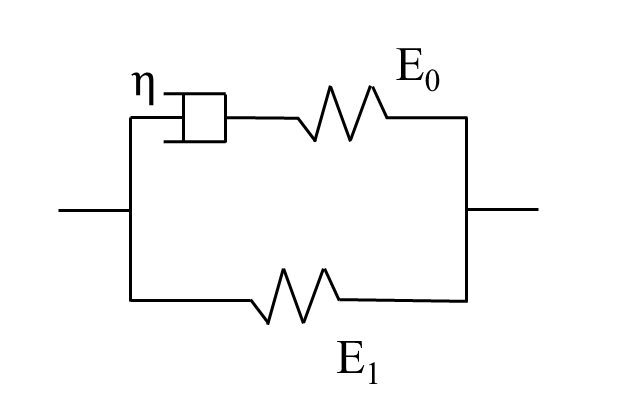
\includegraphics[width=0.5\textwidth]{figs/sls.png}
        \caption{An illustration of Three-element Standard Linear Solid (SLS)
        model. A spring ($E_0$) and a dashpot ($\eta$) are first connected in
        series (Maxwell body). Then the Maxwell body is connected with a spring
        ($E_1$) in parallel.}
    \label{fig:sls}
    \end{figure}

    \begin{table}\label{table:qlv}
        \centering
        \caption{Viscoelastic coefficients and relaxation times used in the
        FEBio simulations.}
        \begin{tabular}{|l|l|l|l|l|l|}
        \hline
        \textbf{Component} & \textbf{$\gamma_i$} & \textbf{$\tau_i$ (s)} & \textbf{$G_\infty$ (kPa)} & \textbf{Poisson's Ratio} & \textbf{$\rho$ (g/cm$^3$)}\\
        \hline
        E2297-AX & 4 & 0.278 & 2 & 0.495 & 1.0 \\
        E2297-BX & 2.75 & 0.167 & 4 & 0.495 & 1.0 \\
        E2297-CX & 4 & 0.083 & 4 & 0.495 & 1.0 \\
        \hline
        \end{tabular}
    \end{table}

    \item[Task 3:] Perform FEA simulations and data analysis

    FEA simulations were performed for 6 different frequencies (50, 100, 150,
    200, 250 and 300 Hz) for each phantom. Time step sizes were scaled
    according to respective excitation frequencies (approximately 1/100 $f$,
    where $f$ is the excitation frequency). All shear wave (phase) velocities
    were estimated by a lateral TTP algorithm~\cite{Pameri2008}.  

\end{description}

All 18 numerical FEBio models are available on QIDW, and example FEBio
simulation templates are available in the GitHub repository:

\url{https://github.com/RSNA-QIBA-US-SWS/QIBA-DigitalPhantoms/tree/master/febio}

The estimated SW phase velocities are displayed in
Figure~\ref{fig:febio_results}. More quantitative numbers are provided in
Table~\ref{table:febio_results} for the sake of completeness. All phase
velocities were estimated from 5 depths (3, 3.25, 3.5, 3.75 and 4 cm) between
the 3--4 cm depth. Recall that the focal depth was set to be at 3 cm in all FEA
simulations. This region appeared to be most stable and therefore was selected
for estimations of SW phase velocities.

\begin{figure}[htb!]
    \centering
    \begin{tabular}{c}
    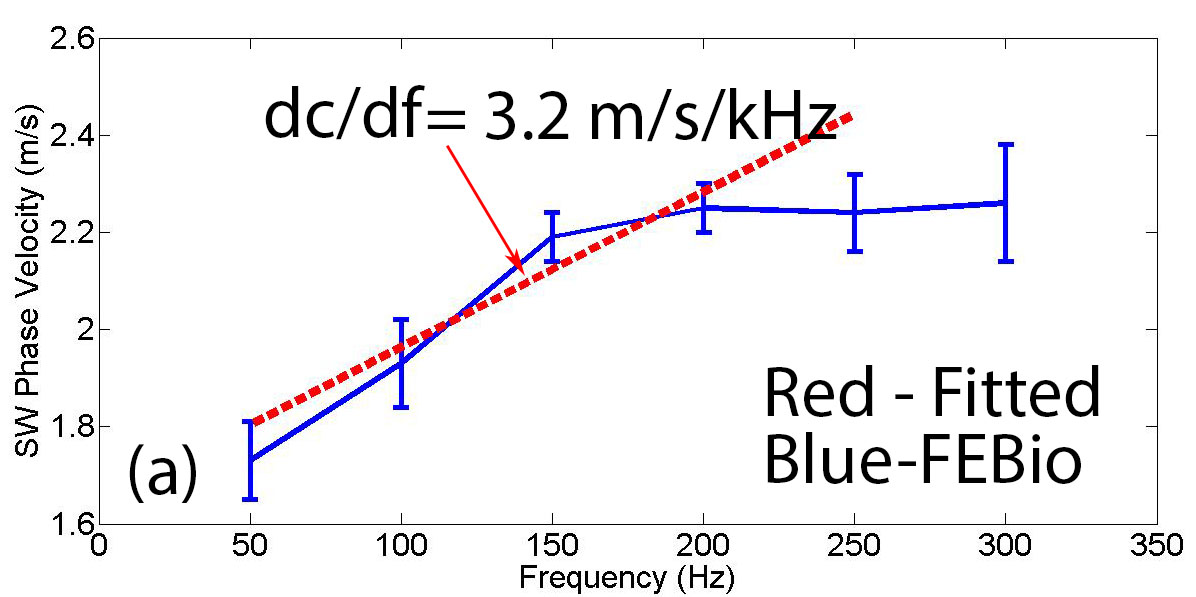
\includegraphics[width=0.5\linewidth]{figs/result1.jpg} \\
    (a) E2297-AX\\
    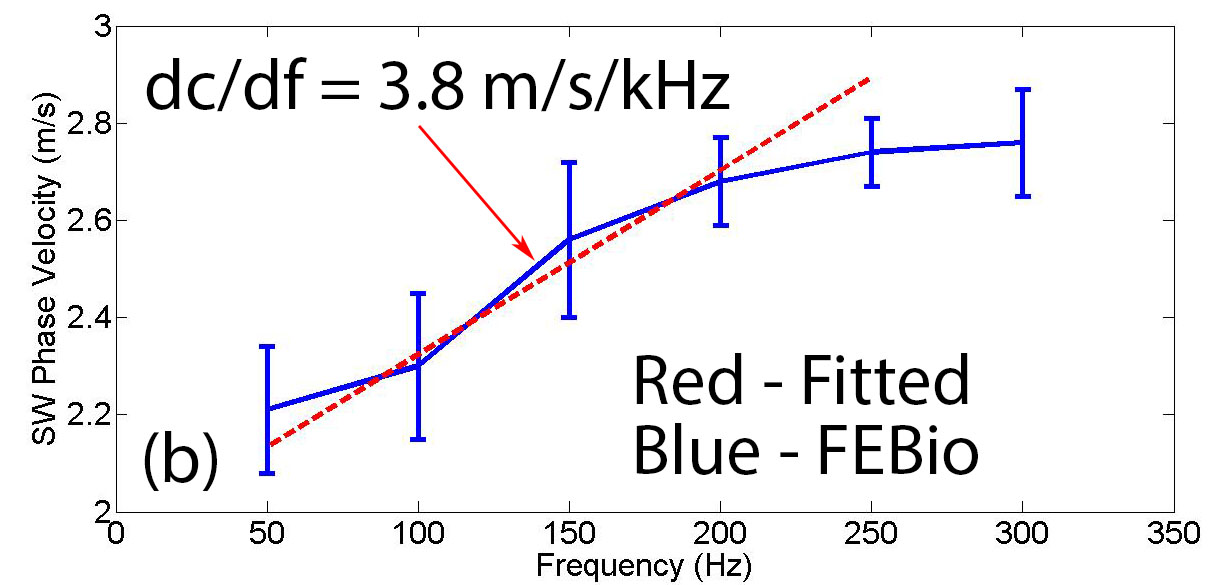
\includegraphics[width=0.5\linewidth]{figs/result2.jpg} \\
    (b) E2297-BX\\
    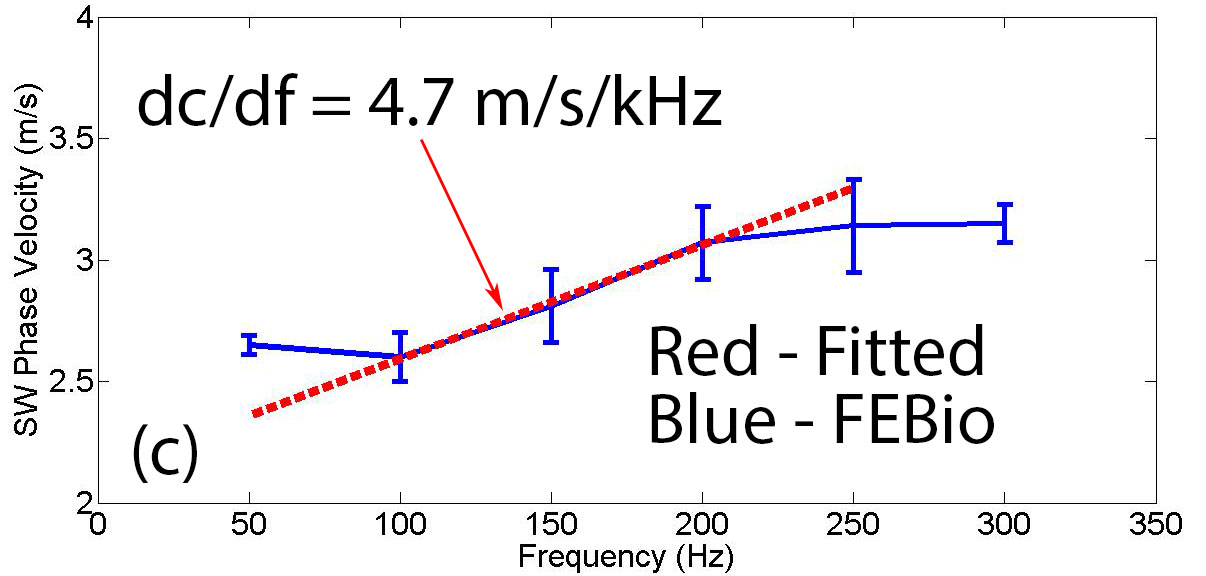
\includegraphics[width=0.5\linewidth]{figs/result3.jpg} \\
    (c) E2297-CX\\
    \end{tabular}
    \caption{Plots of phase velocity vs.\ excitation frequency for three
    different materials: (a) E2297-AX, (b) E2297-BX and (c) E2297-CX\@. Error
    bars denote one standard deviation. All slopes were fit using data points
    between 100--200 Hz.}
\label{fig:febio_results}
\end{figure}

\begin{table}\label{table:febio_results}
    \caption{Tabulated results of estimated phase velocities (m/s) for three
        different materials from 50--300 Hz. The estimated phase velocity is
        displayed as mean $\pm$ one standard deviation.}
    \begin{tabular}{|c|c|c|c|c|c|c|}
        \hline
         & \textbf{50 Hz} & \textbf{100 Hz} & \textbf{150 Hz} & \textbf{200 Hz} & \textbf{250 Hz} & \textbf{300 Hz} \\
         \hline
         \textbf{E2297-AX} & 1.73 $\pm$ 0.08 & 1.93 $\pm$ 0.09 & 2.19 $\pm$ 0.05 & 2.25 $\pm$ 0.05 & 2.24 $\pm$ 0.08 & 2.26 $\pm$ 0.12 \\
         \textbf{E2297-BX} & 2.21 $\pm$ 0.13 & 2.30 $\pm$ 0.15 & 2.56 $\pm$ 0.16 & 2.68 $\pm$ 0.09 & 2.74 $\pm$ 0.07 & 2.76 $\pm$ 0.11 \\
         \textbf{E2297-CX} & 2.65 $\pm$ 0.04 & 2.60 $\pm$ 0.10 & 2.81 $\pm$ 0.15 & 3.07 $\pm$ 0.15 & 3.14 $\pm$ 0.09 & 3.15 $\pm$ 0.08 \\
        \hline
    \end{tabular}
\end{table}

The preliminary results show that FEBio can be used to perform simulations of
shear wave propagation in viscoelastic media. From the 100--200 Hz range, the
frequency dependence of SW phase velocities is clearly visible. Overall, the
simulated results are in a good agreement with the experimental results from
the 100--200 Hz range; however, more investigations are needed to fully
understand the use of FEBio for viscoelastic shear wave simulations.


\subsection{C-Scan Finite Difference Code}
Dr. McAleavey has developed finite difference code solving shear wave
propagation in C-scan planes in viscoelastic media.  This code has been
optimized to run in a GPGPU environment on a desktop workstation and requires
considerably lower computation overhead than the commercial FEA software
packages used to generate the digital phantom data uploaded to QIDW.

Source code for this finite difference algorithm has been shared in the GitHub
repository:

INSERT HYPERLINK HERE

Below is a comparison of the reconstructed viscoelastic material metrics
reconstructed for the 3 configurations used to generate the viscoelastic
digital phantoms:

INSERT TABLE HERE

This code provides accurate solutions in the C-scan plane, but full volumetric
simulated displacement / velocity data are not yet available using this
approach.  This code will continue to evolve through external funding beyond
the scope of QIBA support.
